\documentclass[12pt]{article}
\usepackage{amsmath,amssymb}
\setlength{\oddsidemargin}{0in}
\setlength{\evensidemargin}{0in}
\setlength{\textheight}{9in}
\setlength{\textwidth}{6.5in}
\setlength{\topmargin}{-0.5in}
\usepackage{enumitem}
\usepackage[table]{xcolor}
\usepackage{graphicx}
\usepackage{listings}
\newcommand{\Adv}{{\mathbf{Adv}}}       
\newcommand{\prp}{{\mathrm{prp}}}             
\newcommand{\calK}{{\cal K}}
\newcommand{\outputs}{{\Rightarrow}}

% Use \textbf{Solution:}\\ to begin your solution.

%%%%%%%%%%%%%%%%%%%%%%%%%%%%%%%%%%%%%%%%%%%%%%%%%%%%%%%%%%%%%%%%%%%%%%%%%%%
\title{\bf Math 151A: Problem Set 1}
\date{4/14/2023}
\author{\bf Owen Jones}

\begin{document}
\maketitle

%%%%%%%%%%%%%%%%%%%%%%%%%%%%%%%%%%%%%%%%%%%%%%%%%%%%%%%%
\begin{enumerate}[label=\bfseries Problem \arabic*:]


    %%%%%%%%%%%%%%%%%%%%%%%%%%%%%%
    
    \item \textbf{(T) Taylor's Theorem}\\
    Let $f(x)=e^{2x}$ for $x\in[0,2]$.
    
    \begin{itemize} 
    \item[a)] Find Taylor's polynomial of degree-$2$, i.e. $P_2(x)$, around the point $x_0=0$ and use it to approximate the value of $f(1.5)$, i.e. $f(1.5)\approx P_2(1.5)$. 
    
    \item[b)]  What is the error as a function of $\xi(x)$ when $x=1.5$ (specify the domain for $\xi(1.5)$)?
    
    \item[c)]  What is the actual error (in magnitude)?
    
    \end{itemize}
    
    \textbf{Solution:}

    \begin{itemize}
    \item[a)] $P_2(x)=1+2x+2x^2 \Rightarrow f(1.5)\approx P_2(1.5)=8.5$
    
    \item[b)] $R_2(x)=\frac{f'''(\xi(x))x^3}{6}=\frac{4e^{2\xi(x)}x^3}{3}$ $\Rightarrow$ $R_2(1.5)=\frac{4e^{2\xi(1.5)}1.5^3}{3}$ $\xi(1.5)\in(0,1.5)$

    \item[c)] $R_2(1.5)=e^3-8.5\approx11.5855$

    \end{itemize}

    \newpage
    %%%%%%%%%%%%%%%%%%%%%%%%%%%%%%
    \item \textbf{(T) Bisection Method}\\
    Let $f(x)=\sqrt{\pi\, x}-\cos(\pi\, x)$  over the interval $[0,1]$.  We would like to find $p$ such that $f(p)=0$.
    \begin{itemize}
    \item[a)] Show that the bisection method applied to this problem converges (apply the theorem from class).   
    \item[b)] How many iterations are needed to have a $10^{-q}$-accurate approximation to the true root where $q>1$? Write your answer in the form $n\geq C q$ where $C$ is an explicit constant that you need to provide.  
     
    \end{itemize}
    
    \textbf{Solution:}

    \begin{itemize}
    \item[a)] Applying the theorem from class, $f$ is continuous over $[0,1]$ and $f(0) \cdot f(1)<0$. Thus, $\exists p\in(0,1)$ s.t $f(p)=0$. $f(x)$ over the interval $[0.1]$ is strictly monotonically increasing, so $p$ is unique.
    
    \item[b)] $|p_n-p|\le2^{-n}\le10^{-q}$ $\Rightarrow$ $n \ge \log_2(10)q$

    \end{itemize}
    
    \newpage
    %%%%%%%%%%%%%%%%%%%%%%%
    \item \textbf{(C) Bisection Method}\\
    Find a $10^{-5}$-accurate approximation to $\sqrt[4]{25}$ using the Bisection Algorithm. To do so, you will need to define a function $f(x)$ whose root is $\sqrt[4]{25}$. The function $f(x)$ must only use simple operations: multiplication and addition/subtraction. Use the corollary from class to determine the number of steps required to achieve the given accuracy.
    
    \textbf{Solution:} \newline
    Applying the theorem from class, $f(x)=x^4-25$ which is continuous over $[2,3]$ and $f(2)\cdot f(3)<0 \Rightarrow \exists p \in (2,3)$ s.t $f(p)=0$\newline
    $f'(x)>0$ over the interval $[2,3]$, so $f$ will only intersect with the $x-axis$ at 1 point. Thus, $p$ is unique.\\
    $a_0=2$ $b_0=3$ $p=\sqrt[4]{25}$ \newline
    %$p_n=\frac{1}{2}(a_{n-1}+b_{n-1})$\newline
    $|p_n-p|\le \frac{3-2}{2^n}$\\
    By the corollary from class, $\frac{1}{2^n}<10^{-5} \Rightarrow n=17>log_2(\frac{1}{10^{-5}})$\newline
    $p_{17}=2.236061096191406$ which is within $10^{-5}$ of $\sqrt[4]{25}$ $(|p_{17}-p|\approx 6.88\cdot 10^{-6})$\newline
    \begin{figure}[h!]
        \centering
        \begin{minipage}{.5\textwidth}
            \centering
            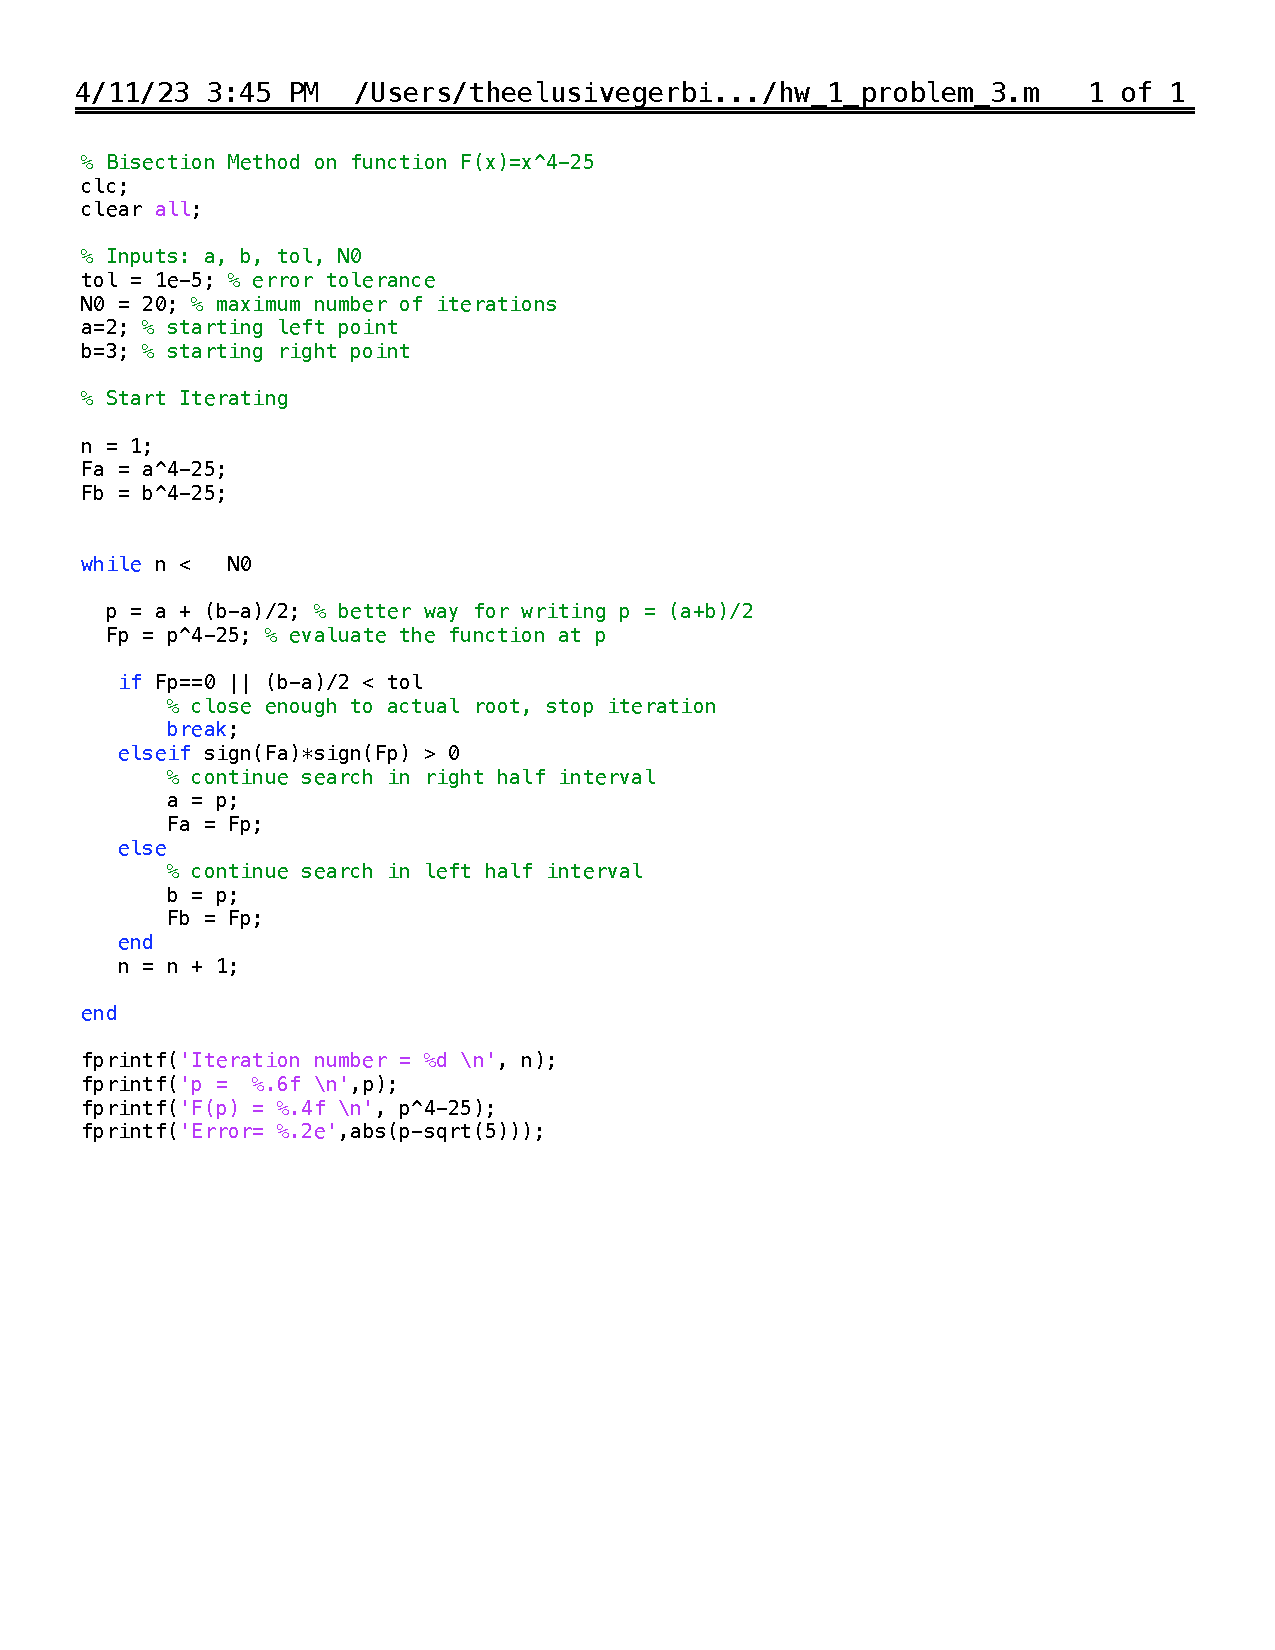
\includegraphics[width=\linewidth]{hw_1_problem_3.pdf}  
        \end{minipage}%
        \begin{minipage}{.5\textwidth}
            \centering
            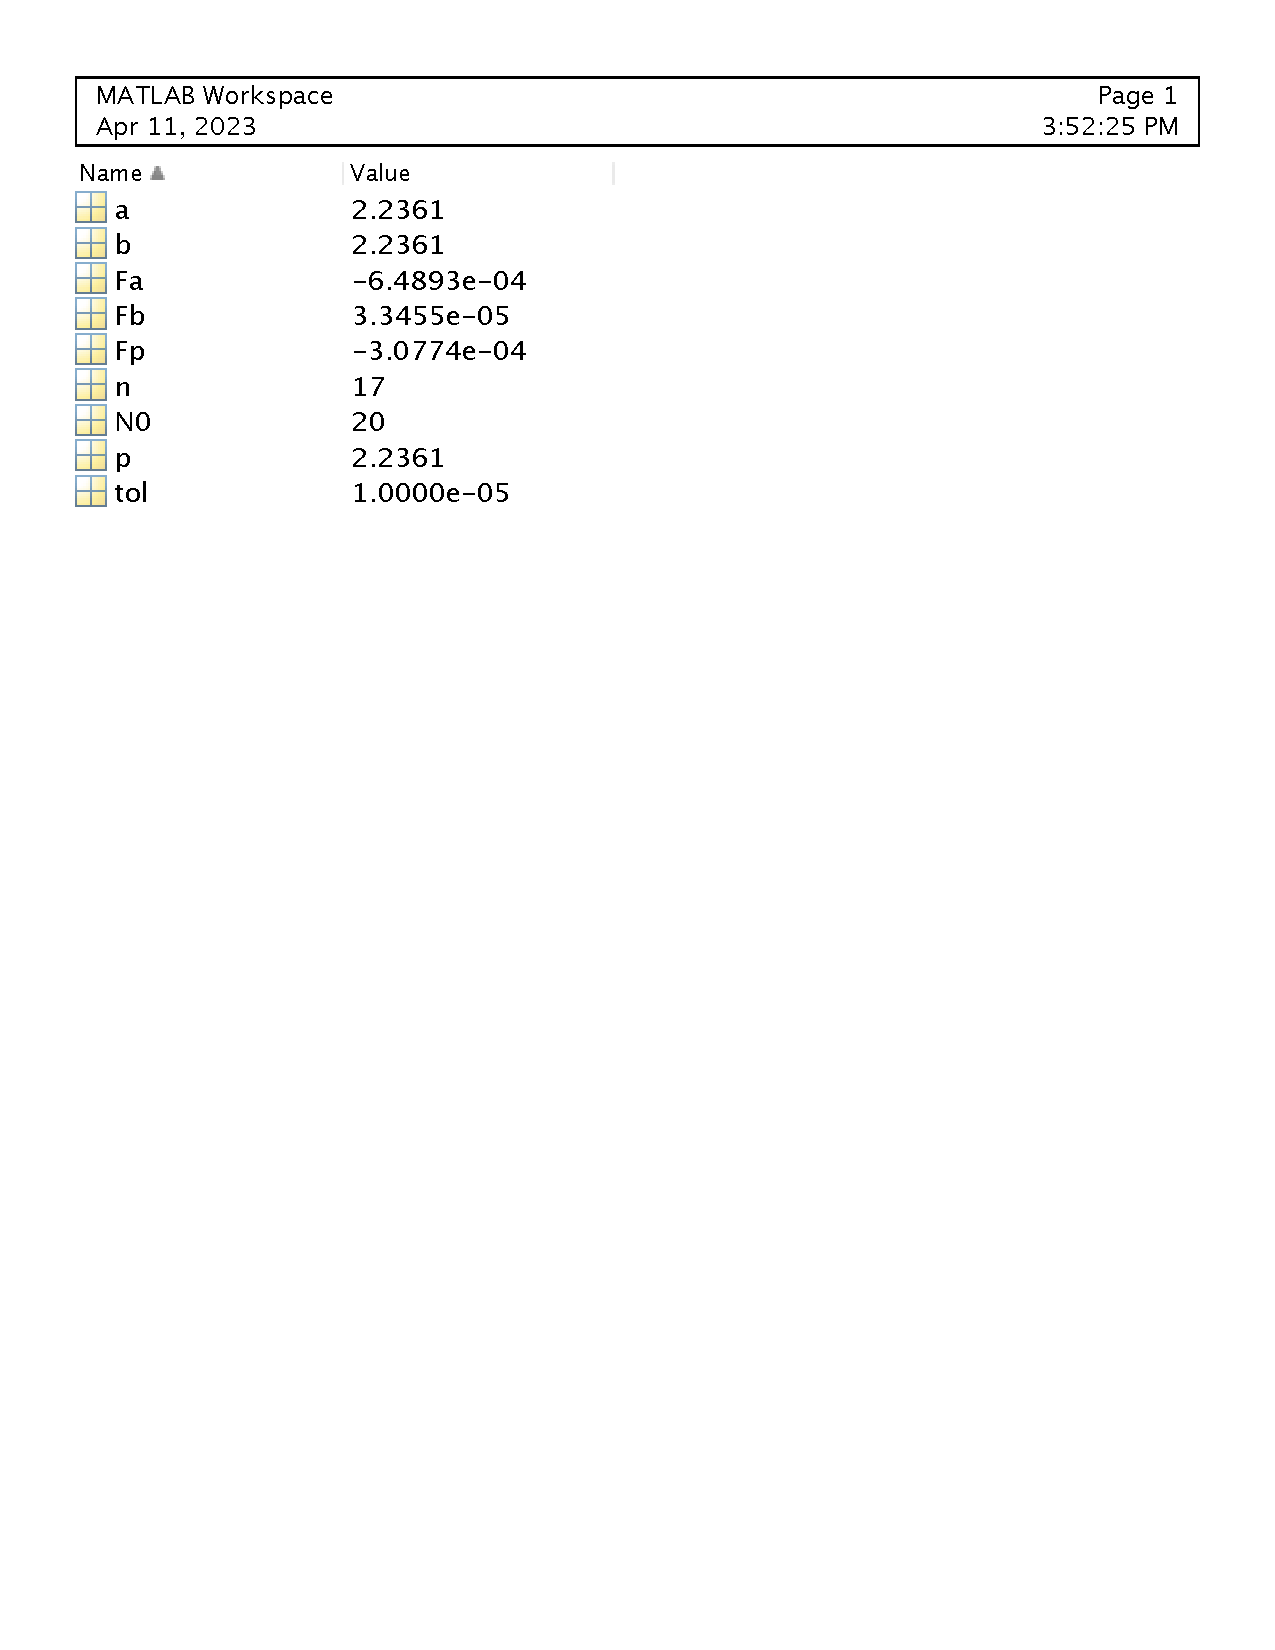
\includegraphics[width=\linewidth]{variables.pdf}
        \end{minipage}%
    \end{figure}
    \newpage
    %%%%%%%%%%%%%%%%%%%%%%%
    \item \textbf{(T) Bisection Method}\\
    You will show that the bisection method may not converge monotonically. Provide a continuous function $f(x)$ and an interval $[a,b]$ so that the error at the $k$-th step, denoted $E_{k}=|p_k-p|$, increases between some iterations although the sequence $p_k$ converges to the unique root. To receive credit for this problem, you must justify your answer and prove that your example is convergent.
    
    \textbf{Solution:} \newline
    $f(x)=x-0.124$ on the interval $[-1,1]$. Let $p_k=\frac{1}{2}(a_{k-1}+b_{k-1})$ and $a_0=-1,b_0=1$. We define $E_k=|f(p_k)|=|p_k-0.124|$. \newline
    Given $f$ is continuous over $[-1,1]$ and $f(-1) \cdot f(1)<0$ $\exists p\in(-1,1)$ s.t $f(p)=0$\\
    $f'(x)>0$ over the interval $[-1,1]$, so $f$ will only intersect with the $x-axis$ at 1 point. Thus, $p$ is unique.\\
    $E_1=0.124,E_2=0.376,E_3=0.126,E_4=0.001...$ \newline
    Since $E_2>E_3>E_1$ the sequence does not converge monotonically.
    
    %WTS $\displaystyle{\lim_{k \to \infty}}p_k=0.124$ \newline
    %$\forall \epsilon$ choose $N$ to be large enough s.t $2^{1-N} \le \epsilon$. $(N\ge log_2{\frac{2}{\epsilon}})$\newline 
    %If $k>N$ \newline
    %$\Rightarrow |p_k-0.124|\le 2^{1-k}<2^{1-N}$ \newline
    %Because $2^{1-N}\le \epsilon$ \newline
    %$\Rightarrow |p_k-0.124|<\epsilon$ \newline
    %Hence, $\displaystyle{\lim_{k \to \infty}}p_k=0.124$\\
   
 
     
    \newpage 
    %%%%%%%%%%%%%%%%%%%%%%%
    \item \textbf{(T) Stopping Criteria for General Root-Finding Algorithms}\\
    Assume that we have a sequence $p_n$ for $n=1,2,...$ that is generated by an algorithm in order to find the root of a function $f(x)$. Let $\epsilon$ be the prescribed tolerance used to stop the iterative process. 
    
    You may use, without proof, that  $\sum_{k=1}^n \frac{1}{k}$ diverges as $n\rightarrow \infty$.
    
    
    
    \begin{itemize}
    \item[a)] Consider the stopping criterium $|p_{n}-p_{n-1}|< \epsilon$ for $n>2$. Show that $p_n=\sum_{k=1}^n \frac{1}{k}$ satisfies the criterium when $n\geq\frac{1}{\epsilon}$; however, $p_n \rightarrow \infty$  (thus the sequence does not converge to a finite value).
    
    
    \item[b)] Consider the stopping criterium $\frac{|p_{n}-p_{n-1}|}{|p_n|}< \epsilon$ for $n>2$ and $p_n\neq 0$. Show that $p_n=\sum_{k=1}^n \frac{1}{k}$ satisfies the criterium; however, $p_n \rightarrow \infty$ (thus the sequence does not converge to a finite root).
    
     
    \item[c)] Let  $f(x):=(x-1)^{10}$, whose root is $p=1$, and define the sequence $p_n=1+\frac{1}{n}$. Note that $p_n$ goes to the root in the limit. Show that the stopping criterium $|f(p_n)| < 10^{-3}$ is achieved for all $n>1$ but $|p-p_n|\leq 10^{-3}$ requires $n>1000$.
     
     
    \end{itemize}
    
    \textbf{Solution:}

    \begin{itemize}
    \item[a)] If $n>\frac{1}{\epsilon}$ \newline
    $\Rightarrow\epsilon>\frac{1}{n}=|\frac{1}{n}+\sum_{k=1}^{n-1}\frac{1}{k}-\sum_{k=1}^{n-1}\frac{1}{k}|=|\sum_{k=1}^{n}\frac{1}{k}-\sum_{k=1}^{n-1}\frac{1}{k}|$ \newline
    Hence, the stopping criteria is met for $n>\frac{1}{\epsilon}$. However, since $\sum_{k=1}^{\infty}\frac{1}{k}$ diverges, $\displaystyle{\lim_{k \to \infty}}p_k=\infty$.
    \item[b)] $|p_n|=|\sum_{k=1}^{n}\frac{1}{k}|\ge|\sum_{k=1}^{n}\frac{1}{n}|=1\Rightarrow \frac{1}{|p_n|}\le 1$\\
    It follows $\frac{|p_{n}-p_{n-1}|}{|p_n|}\le\frac{|p_{n}-p_{n-1}|}{\sum_{k=1}^{n}\frac{1}{n}}=\frac{|p_{n}-p_{n-1}|}{\frac{n}{n}}=|p_{n}-p_{n-1}|$ \newline
    By part a, $n>\frac{1}{\epsilon}\Rightarrow|p_{n}-p_{n-1}|<\epsilon$ \newline
    Because $\frac{|p_{n}-p_{n-1}|}{|p_n|}\le |p_{n}-p_{n-1}|\Rightarrow\frac{|p_{n}-p_{n-1}|}{|p_n|}<\epsilon$ \newline
    Hence, the stopping criteria is met for $n>\frac{1}{\epsilon}$. However, since $\sum_{k=1}^{\infty}\frac{1}{k}$ diverges, $\displaystyle{\lim_{k \to \infty}}p_k=\infty$.
    \item[c)] $|p_n-p|=|1+\frac{1}{n}-1|=\frac{1}{n}<10^{-3}\Rightarrow n>1000$ \newline
    If $10^{\frac{3}{10}}<n\Rightarrow|f(p_n)-f(p)|=\frac{1}{n^{10}}<10^{-3}$

    \end{itemize}
    
    \end{enumerate}

\end{document}